\documentclass[tikz,border=5pt]{standalone}
\usepackage[UTF8]{ctex}
\usepackage{amsmath,amssymb}
\usetikzlibrary{arrows.meta,calc,angles,quotes,positioning,decorations.pathreplacing,decorations.pathmorphing,patterns}
\definecolor{ink}{HTML}{243447}
\definecolor{blue}{HTML}{2765A2}
\definecolor{red}{HTML}{B74739}
\definecolor{green}{HTML}{278365}
\tikzset{line cap=round,line join=round,
body/.style={draw=ink,very thick},
vec/.style={draw=blue,very thick,-{Latex[length=2.3mm]}},
force/.style={draw=red,very thick,-{Latex[length=2.3mm]}},
ray/.style={draw=green!85!black,thick,-{Latex[length=2mm]}},
guide/.style={draw=ink!45,dashed},
dim/.style={draw=ink!75,{Latex[length=1.8mm]}-{Latex[length=1.8mm]}}}
\begin{document}
% 1. question
\begin{tikzpicture}
 \fill[blue!5] (0,-.15) rectangle (4.5,4.2);
 \draw[body,fill=gray!15] (-.08,0) rectangle (.08,4);
 \draw[body] (4.5,-.3)--(4.5,4.2);
 \fill[pattern=north east lines,pattern color=gray!60] (4.5,-.3) rectangle (4.85,4.2);
 \draw[vec] (.25,2)--(1.65,2) node[midway,above] {$u$};
 \draw[dim] (.1,-.6)--(4.5,-.6) node[midway,fill=white] {$a$};
 \fill (0,0) circle(2.2pt) node[below left] {$A$};
 \fill (4.5,0) circle(2.2pt) node[below right] {$B$};
 \fill (4.5,2.9) circle(2.2pt) node[right=7pt] {$C$};
 \draw[dim] (4.18,0)--(4.18,2.9) node[midway,left] {$x$};
 \node[left] at (-.15,2.8) {钢管};
 \node at (2.7,3.5) {水};
 \node[right] at (4.95,1.2) {河岸};
\end{tikzpicture}
% 2. solution
\begin{tikzpicture}
 \begin{scope}[scale=.68]
  \foreach \j/\u/\lab in {0/.4/{u<c},1/1/{u=c},2/1.7/{u>c}}{
   \begin{scope}[xshift=\j*8cm]
    \pgfmathsetmacro{\t}{3/max(1,\u)}
    \draw[body] (3,-.2)--(3,5.8);
    \foreach \q in {0,.33,.66,1}{
     \pgfmathsetmacro{\ta}{\q*\t}
     \pgfmathsetmacro{\rad}{\t-\ta}
     \draw[blue!65] (\u*\ta,1.5*\ta) circle[radius=\rad cm];
     \fill[red] (\u*\ta,1.5*\ta) circle(2.3pt);
    }
    \draw[guide] (0,0)--(\u*\t,1.5*\t);
    \fill (0,0) circle(2pt) node[below left] {$A$};
    \fill (3,0) circle(2pt) node[right] {$B$};
    \node at (1,6.4) {$\lab$};
    \ifnum\j=0
     \node at (1,-3.8) {$\tau_*=0$};
    \fi
    \ifnum\j=1
     \draw[red,line width=2pt] (3,0)--(3,4.5);
     \node at (1,-3.8) {整段同时触岸};
    \fi
    \ifnum\j=2
     \fill[red] (3,1.5*\t) circle(3.3pt) node[right] {$C$};
     \node at (1,-3.8) {$\tau_*=a/u$};
    \fi
   \end{scope}
  }
 \end{scope}
\end{tikzpicture}
% 3. question
\begin{tikzpicture}
 \fill[blue!7] (0,0) rectangle (3,2);
 \fill[red!5] (3.15,0) rectangle (6.15,2);
 \draw[body] (8,0)--(0,0)--(0,2)--(8,2);
 \draw[body,fill=gray!30] (3,0) rectangle (3.15,2);
 \draw[body,fill=gray!15] (6.15,0) rectangle (6.3,2);
 \draw[guide] (3.08,2)--(3.08,2.55);
 \node[above] at (3.08,2.55) {固定、导热};
 \draw[guide] (6.23,0)--(6.23,-.55);
 \node[below] at (6.23,-.55) {可动、绝热};
 \node[align=center] at (1.5,1) {$n,V_0$\\$p_0,T_0$};
 \node[align=center] at (4.65,1) {$n,V_0$\\$p_0,T_0$};
 \node at (7.4,1) {$p_0$};
 \draw[force] (4.6,3)--(4.6,2.15) node[midway,right] {$Q_0$};
\end{tikzpicture}
% 4. solution
\begin{tikzpicture}
 \draw[vec] (0,0)--(5.2,0) node[right] {$q/q_\infty$};
 \draw[vec] (0,0)--(0,3.5) node[above] {$nR(T-T_0)/Q_0$};
 \draw[red,very thick] (0,2.85714)--(4.5,1.66667);
 \draw[blue,very thick] (0,0)--(4.5,1.66667);
 \node[right,red] at (1,2.85) {$T_{\mathrm R}$};
 \node[below,blue] at (2.7,.9) {$T_{\mathrm L}$};
 \draw[guide] (4.5,0)--(4.5,1.66667)--(0,1.66667);
 \draw[guide] (2.25,0)--(2.25,2.2619);
 \draw[dim] (2.25,.83333)--(2.25,2.2619) node[midway,right,fill=white] {$1/7$};
 \node[left] at (0,2.85714) {$2/7$};
 \node[left] at (0,1.66667) {$1/6$};
 \node[below] at (2.25,0) {$1/2$};
 \node[below] at (4.5,0) {$1$};
 \begin{scope}[xshift=7.2cm,yshift=.4cm]
  \draw[body] (0,0) rectangle (3.4,1.8);
  \fill[red!5] (0,0) rectangle (2.6,1.8);
  \draw[body] (2.6,0)--(2.6,1.8);
  \draw[guide] (1.8,0)--(1.8,1.8);
  \draw[vec] (2.55,2.2)--(1.85,2.2);
  \node at (1.3,.9) {$p_0$};
  \node[align=center] at (1.7,-.65) {向左传热\\右室等压收缩};
 \end{scope}
\end{tikzpicture}
% 5. question
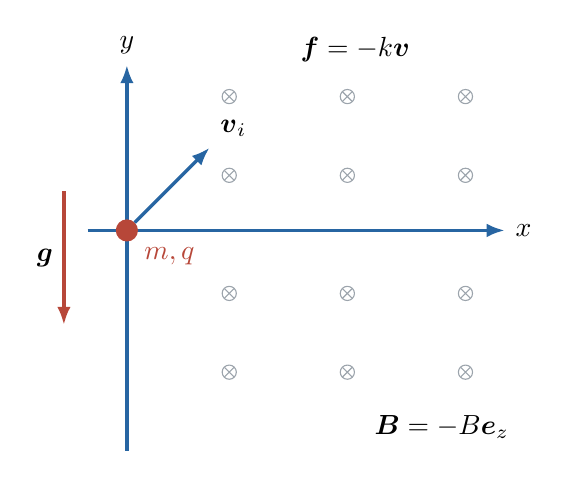
\begin{tikzpicture}
 \draw[vec] (-.5,0)--(4.8,0) node[right] {$x$};
 \draw[vec] (0,-2.8)--(0,2.1) node[above] {$y$};
 \foreach \x in {1.3,2.8,4.3}{
  \foreach \y in {-1.8,-.8,.7,1.7}{
   \draw[ink!45] (\x,\y) circle(.09);
   \draw[ink!45] (\x-.06,\y-.06)--(\x+.06,\y+.06)
   (\x-.06,\y+.06)--(\x+.06,\y-.06);
  }
 }
 \fill[red] (0,0) circle(4pt) node[below right=4pt] {$m,q$};
 \draw[vec] (.1,.1)--(1.05,1.05) node[above right] {$\boldsymbol v_i$};
 \draw[force] (-.8,.5)--(-.8,-1.2) node[midway,left] {$\boldsymbol g$};
 \node at (4,-2.5) {$\boldsymbol B=-B\boldsymbol e_z$};
 \node at (2.9,2.3) {$\boldsymbol f=-k\boldsymbol v$};
\end{tikzpicture}
% 6. solution
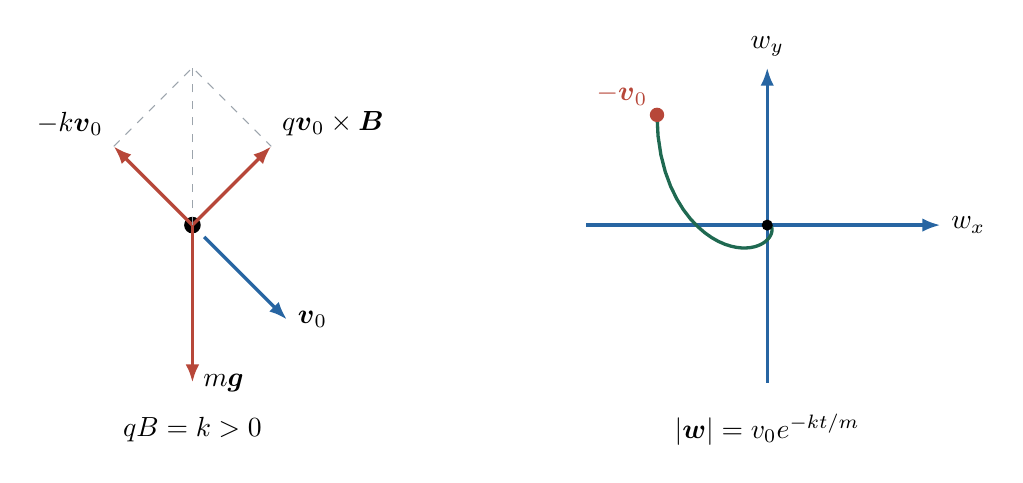
\begin{tikzpicture}
 \begin{scope}[xshift=-3.4cm]
  \fill (0,0) circle(3pt);
  \draw[force] (0,0)--(0,-2) node[right] {$m\boldsymbol g$};
  \draw[force] (0,0)--(-1,1) node[above left] {$-k\boldsymbol v_0$};
  \draw[force] (0,0)--(1,1) node[above right] {$q\boldsymbol v_0\times\boldsymbol B$};
  \draw[guide] (-1,1)--(0,2)--(1,1);
  \draw[guide] (0,0)--(0,2);
  \draw[vec] (.15,-.15)--(1.2,-1.2) node[right] {$\boldsymbol v_0$};
  \node at (0,-2.6) {$qB=k>0$};
 \end{scope}
 \begin{scope}[xshift=3.9cm]
  \draw[vec] (-2.3,0)--(2.2,0) node[right] {$w_x$};
  \draw[vec] (0,-2)--(0,2) node[above] {$w_y$};
  \draw[green!80!black,very thick,samples=160,domain=0:16,variable=\t]
  plot ({1.4*exp(-\t)*(-cos(57.2958*\t)-sin(57.2958*\t))},
        {1.4*exp(-\t)*(-sin(57.2958*\t)+cos(57.2958*\t))});
  \fill[red] (-1.4,1.4) circle(2.6pt) node[above left] {$-\boldsymbol v_0$};
  \fill (0,0) circle(2pt);
  \node at (0,-2.6) {$|\boldsymbol w|=v_0e^{-kt/m}$};
 \end{scope}
\end{tikzpicture}
% 7. question
\begin{tikzpicture}
 \shade[ball color=blue!35] (0,0) circle(1.15);
 \shade[ball color=gray!35] (10,0) circle(.64);
 \draw[body] (1.18,-.12)--(9.25,-.12) (1.18,.12)--(9.25,.12);
 \draw[body] (1.18,0) ellipse(.05 and .12);
 \draw[body,fill=red!20] (9.12,-.3) rectangle (9.33,.3);
 \draw[vec] (-.5,-1.65)--(10.8,-1.65) node[right] {$x$};
 \draw[guide] (0,0)--(0,-1.65) (10,0)--(10,-1.65);
 \fill (0,0) circle(2pt); \fill (10,0) circle(2pt);
 \fill[red] (.72,0) circle(2.5pt);
 \node[above] at (0,1.15) {地球};
 \node[above] at (10,.65) {月球};
 \node[above] at (9.2,.45) {$M_0$};
 \node[below] at (0,-1.65) {$0$};
 \node[below] at (10,-1.65) {$r$};
 \draw[dim] (1.2,-.75)--(9.25,-.75);
 \node[below] at (1.2,-.75) {$a=R_E$};
 \node[below] at (8.7,-.75) {$b=r-R_M$};
 \node[above left] at (.72,.1) {$x_c$};
 \node at (5.4,1.0) {与地月连线共转};
 \node at (5.4,-2.5) {距离与球体大小不按同一比例};
\end{tikzpicture}
% 8. solution
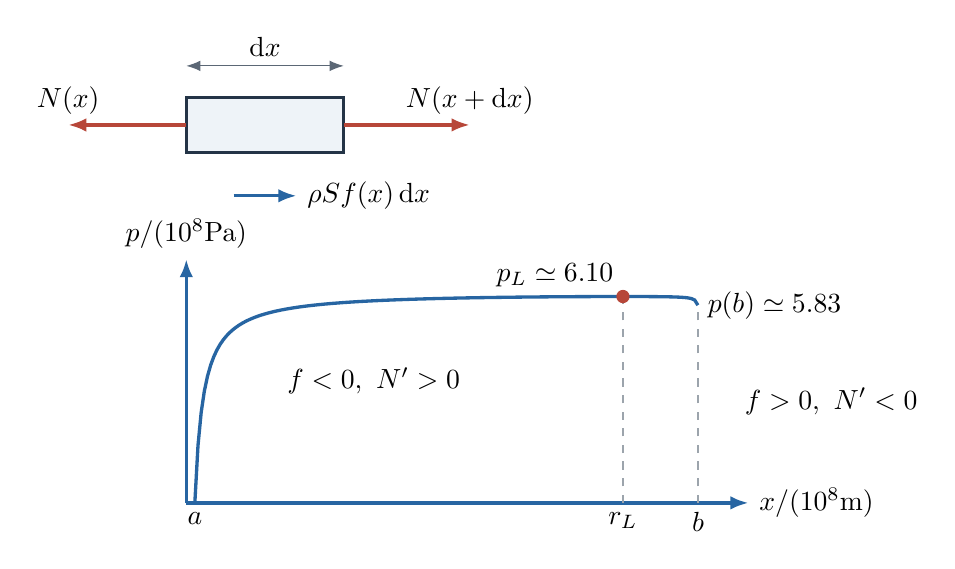
\begin{tikzpicture}
 \begin{scope}[yshift=4.8cm]
  \draw[body,fill=blue!8] (0,-.35) rectangle (2,.35);
  \draw[force] (0,0)--(-1.5,0) node[above] {$N(x)$};
  \draw[force] (2,0)--(3.6,0) node[above] {$N(x+\mathrm dx)$};
  \draw[vec] (.6,-.9)--(1.4,-.9) node[right] {$\rho S f(x)\,\mathrm dx$};
  \draw[dim] (0,.75)--(2,.75) node[midway,above] {$\mathrm dx$};
 \end{scope}
 \begin{scope}[x=1.7cm,y=.43cm]
  \draw[vec] (0,0)--(4.2,0) node[right] {$x/(10^8\mathrm m)$};
  \draw[vec] (0,0)--(0,7.2) node[above] {$p/(10^8\mathrm{Pa})$};
  \draw[blue,very thick,samples=160,domain=.0637:3.8226]
  plot (\x,{6.262931903-.398866/\x-.00490245/(3.84-\x)-.0035479457*(\x-.046624267)^2});
  \draw[guide] (3.261937,0)--(3.261937,6.095493);
  \fill[red] (3.261937,6.095493) circle(2.4pt);
  \node[above left] at (3.261937,6.095493) {$p_L\simeq6.10$};
  \draw[guide] (3.8226,0)--(3.8226,5.826251);
  \node[right] at (3.8226,5.826251) {$p(b)\simeq5.83$};
  \node[below] at (3.261937,0) {$r_L$};
  \node[below] at (.0637,0) {$a$};
  \node[below] at (3.8226,0) {$b$};
  \node at (1.4,3.6) {$f<0,\ N'>0$};
  \node[right] at (4.1,3.0) {$f>0,\ N'<0$};
 \end{scope}
\end{tikzpicture}
% 9. question
\begin{tikzpicture}
 \draw[body] (-1,0)--(1.6,0);
 \fill[pattern=north east lines,pattern color=gray] (-1,0) rectangle (1.6,.2);
 \draw[body] (0,0)--(0,-1.65);
 \draw[red,very thick,decorate,decoration={zigzag,segment length=5pt,amplitude=2pt}] (0,-1.65)--(0,-4.78);
 \fill[ink] (0,-4.95) circle(.17) node[right=7pt] {$m$};
 \draw[blue,thick] (-1.1,-4.95)--(2.5,-4.95);
 \node[right] at (2.5,-4.95) {水面};
 \draw[vec] (-1.6,.1)--(-1.6,-5.4) node[below] {$y$};
 \draw[guide] (-.5,-1.65)--(2,-1.65);
 \draw[guide] (-.5,-2.75)--(2,-2.75);
 \node[right] at (2,-1.65) {$y=L$};
 \node[right] at (2,-2.75) {$y=y_e$};
 \node[right] at (1.7,-4.7) {$y=h$};
 \draw[dim] (1.05,0)--(1.05,-1.65) node[midway,right] {$L$};
 \draw[dim] (1.05,-1.65)--(1.05,-4.95) node[midway,right] {$h-L$};
\end{tikzpicture}
% 10. solution
\begin{tikzpicture}
 \begin{scope}[x=.65cm,y=1.1cm]
  \draw[vec] (0,0)--(9.8,0) node[right] {$y/(10\,\mathrm m)$};
  \draw[vec] (0,-2.3)--(0,1.55) node[above] {$a/g$};
  \draw[blue,very thick] (0,1)--(3,1)--(9,-2);
  \foreach \x in {3,5,9}{\draw[guide] (\x,0)--(\x,{min(1,2.5-.5*\x)});\node[below] at (\x,0) {$\x$};}
  \node[left] at (0,1) {$1$}; \node[left] at (0,-2) {$-2$};
  \node at (1.4,-.75) {松绳};
  \node at (6.6,1.2) {张紧};
 \end{scope}
 \begin{scope}[xshift=10cm]
  \draw[guide] (0,0) circle(2);
  \draw[vec] (-2.3,0)--(2.5,0) node[right] {$v/(A\omega)$};
  \draw[vec] (0,-2.3)--(0,2.5) node[above] {$z/A$};
  \draw[red,very thick,-{Latex}] (1.732,-1) arc[start angle=-30,end angle=90,radius=2];
  \fill[red] (1.732,-1) circle(2.5pt) node[right] {张紧初态};
  \fill[red] (0,2) circle(2.5pt) node[above left] {最低点};
  \draw[guide] (0,0)--(1.732,-1);
  \node at (.45,.8) {$\Delta\varphi=2\pi/3$};
  \node[left] at (0,-1) {$-1/2$};
  \node at (0,-3.0) {$z=y-y_e$};
 \end{scope}
\end{tikzpicture}
% 11. question
\begin{tikzpicture}
 \draw[vec] (-.2,-1.5)--(8,-1.5) node[right] {$x$};
 \fill[red!20,draw=red,thick] (1,0) circle(.35);
 \fill[blue!15,draw=blue,thick] (6,0) circle(.6);
 \draw[vec] (1.5,0)--(3.1,0) node[midway,above] {$p_i$};
 \node[above] at (1,.5) {$\alpha$};
 \node[below] at (1,-.4) {$m,q_1,E_0$};
 \node[above] at (6,.75) {金核};
 \node[below] at (6,-.65) {$M,q_2$};
 \node at (6,1.8) {初始静止、可反冲};
\end{tikzpicture}
% 12. solution
\begin{tikzpicture}
 \begin{scope}
  \node at (2.2,2) {质心系};
  \fill[red!20,draw=red] (0,1) circle(.22);
  \fill[blue!15,draw=blue] (4.4,1) circle(.38);
  \draw[vec] (.3,1)--(1.55,1) node[midway,above] {$p_*$};
  \draw[vec] (3.95,1)--(2.7,1) node[midway,above] {$-p_*$};
  \fill[red!20,draw=red] (1.45,-.65) circle(.22);
  \fill[blue!15,draw=blue] (2.95,-.65) circle(.38);
  \draw[dim] (1.45,-1.4)--(2.95,-1.4) node[midway,below] {$d$};
  \node at (2.2,-2.0) {$v_{\mathrm{He}}^*=v_{\mathrm{Au}}^*=0$};
 \end{scope}
 \begin{scope}[xshift=7cm]
  \draw[vec] (0,0)--(4.8,0) node[right] {$r$};
  \draw[vec] (0,0)--(0,3.4) node[above] {$U$};
  \draw[blue,very thick,domain=.65:4.5,samples=70] plot(\x,{2/\x});
  \draw[red,thick] (0,1.5)--(4.5,1.5) node[right] {$\mathcal E_*-(m+M)c^2$};
  \draw[guide] (1.3333,0)--(1.3333,1.5);
  \node[below] at (1.3333,0) {$d$};
  \node at (3.1,.2) {$Kq_1q_2/r$};
 \end{scope}
\end{tikzpicture}
% 13. question: 3D water tank, observation perpendicular to illumination
\begin{tikzpicture}
 \fill[blue!8] (0,0)--(6,0)--(6,2.2)--(0,2.2)--cycle;
 \fill[blue!4] (0,2.2)--(1,3)--(7,3)--(6,2.2)--cycle;
 \draw[body] (0,0)--(6,0)--(6,2.2)--(0,2.2)--cycle;
 \draw[body] (6,0)--(7,.8)--(7,3)--(6,2.2) (0,2.2)--(1,3)--(7,3);
 \draw[guide] (1,3)--(1,.8)--(7,.8) (0,0)--(1,.8);
 \draw[force] (-1.8,1.2)--(2.5,1.2) node[pos=.16,above] {激光};
 \draw[body,fill=white] (2.7,1.2) circle(.18);
 \node[below] at (2.7,.95) {气泡};
 \draw[guide] (2.7,1.2)--(2.7,5.6);
 \draw[blue,very thick,{Latex}-{Latex}] (1.65,4.15)--(3.75,4.15);
 \draw[body,fill=gray!15] (2.1,5.25) rectangle (3.3,5.65);
 \node[right] at (3.4,5.5) {相机};
 \draw[ray] (2.7,1.2)--(2.4454,2.2)--(1.8,4.15)--(2.6,5.25);
 \draw[ray] (2.7,1.2)--(2.9546,2.2)--(3.6,4.15)--(2.8,5.25);
 \draw[guide] (2.4454,2.2)--(2.7,1.43077)--(2.9546,2.2);
 \fill[red] (2.7,1.43077) circle(2pt) node[right=6pt] {视位置};
 \draw[dim] (4.25,1.43077)--(4.25,4.15) node[midway,right] {$L$};
 \draw[dim] (1.65,4.6)--(3.75,4.6) node[midway,above] {$D$};
 \node at (5,1.2) {$n=1.3$};
\end{tikzpicture}
% 14. solution: physically traced paths (radius=2)
\begin{tikzpicture}
 \coordinate (O) at (0,0);
 \coordinate (P) at (-1.414214,1.414214);
 \coordinate (E) at (-1.784895,-.902302);
 \coordinate (H) at (1.414214,-1.414214);
 \coordinate (Q) at (.902302,1.784895);
 \draw[body,fill=blue!3] (O) circle(2);
 \draw[guide] (-2.3,0)--(2.4,0) (0,-2.3)--(0,2.6);
 \draw[guide] (O)--(P) (O)--(E) (O)--(H) (O)--(Q);
 \draw[force] (-3.5,1.414214)--(P);
 \draw[force] (P)--(-1.414214,3.4);
 \draw[ray] (-3.5,-.902302)--(E);
 \draw[ray] (E)--(H);
 \draw[ray] (H)--(Q);
 \draw[ray] (Q)--(.902302,3.4);
 \draw[dim] (-1.414214,3.7)--(.902302,3.7) node[midway,above] {$s$};
 \foreach \name in {P,E,H,Q}{\fill[ink] (\name) circle(2.4pt);}
 \node[above left] at (P) {$P$}; \node[right] at (Q) {$Q$};
 \node[below left] at (E) {$E$}; \node[below right] at (H) {$H$};
 \node[below left] at (O) {$O$};
 \draw (0,.65) arc[start angle=90,end angle=135,radius=.65];
 \node at (-.4,.85) {$\alpha$};
 \draw (0,1.1) arc[start angle=90,end angle=63.1824,radius=1.1];
 \node at (.3,1.28) {$\beta$};
 \node at (-1,.35) {空气};
 \node at (-2.8,-2) {水};
 \begin{scope}[xshift=5.1cm,yshift=.2cm]
  \draw[vec] (-.4,0)--(3.6,0) node[right] {$\theta_{\mathrm a}$};
  \draw[blue,thick,domain=0:3.2,samples=100] plot(\x,{.8+.65*cos(720*\x/3.2)});
  \draw[dim] (.4,1.8)--(2,1.8) node[midway,above] {$\Delta\theta_{\mathrm a}=\lambda_0/s$};
  \node[align=center] at (1.6,-1.0) {$s=R_b(\sin\alpha+\sin\beta)$\\$N\simeq sD/(\lambda_0L)$};
 \end{scope}
\end{tikzpicture}
% 15. question: C7 with first- and second-neighbor edges
\begin{tikzpicture}
 \foreach \i in {0,...,6}{
  \coordinate (A\i) at ({115+\i*360/7}:2.65);
 }
 \foreach \i in {0,...,6}{
  \pgfmathtruncatemacro{\j}{mod(\i+1,7)}
  \pgfmathtruncatemacro{\k}{mod(\i+2,7)}
  \draw[body] (A\i)--(A\j);
  \draw[blue,thick] (A\i)--(A\k);
 }
 \foreach \i in {0,...,6}{
  \fill[ink] (A\i) circle(3pt);
  \node at ({115+\i*360/7}:3.05) {$A_{\i}$};
 }
 \node at (0,-3.6) {每条支路 $1\,\Omega$；交叉处不连接};
\end{tikzpicture}
% 16. solution
\begin{tikzpicture}
 \coordinate (O) at (0,0); \coordinate (U) at (3,1.8);
 \coordinate (V) at (3,-1.8); \coordinate (W) at (6,0);
 \foreach \a/\b/\rr in {O/U/{r_0/2},O/V/{r_0/2},U/V/{r_0/2},U/W/{r_0/2},V/W/{r_0/4}}{
  \draw[body] (\a)--(\b) node[midway,fill=white,inner sep=2pt] {$\rr$};
 }
 \foreach \p in {O,U,V,W}{\fill[ink] (\p) circle(2.8pt);}
 \node[above left] at (O) {$A_0$};
 \node[above right=5pt] at (U) {$U:(A_1,A_6)$};
 \node[below right=5pt] at (V) {$V:(A_2,A_5)$};
 \node[above right=7pt] at (W) {$W:(A_3,A_4)$};
 \draw[vec] (-1.5,0)--(-.12,0) node[midway,above] {$I$};
 \draw[force] (3,1.95)--(3,3.05) node[above] {$I/3$};
 \draw[force] (3,-1.95)--(3,-3.05) node[below] {$I/3$};
 \draw[force] (6.2,0)--(7.2,0) node[midway,below=3pt] {$I/3$};
 \draw[vec] (.35,.9)--(1.15,1.38) node[midway,above left] {$I_a$};
 \draw[vec] (3.45,.75)--(3.45,-.75) node[midway,right] {$I_b$};
 \node[align=center] at (3,-4.1) {叠加后：$A_0$ 流入 $7I/6$，$A_j$ 流出 $7I/6$\\其余节点外部电流为零};
\end{tikzpicture}
\end{document}
